% Options for packages loaded elsewhere
\PassOptionsToPackage{unicode}{hyperref}
\PassOptionsToPackage{hyphens}{url}
%
\documentclass[
  8pt,
]{article}
\usepackage{lmodern}
\usepackage{amssymb,amsmath}
\usepackage{ifxetex,ifluatex}
\ifnum 0\ifxetex 1\fi\ifluatex 1\fi=0 % if pdftex
  \usepackage[T1]{fontenc}
  \usepackage[utf8]{inputenc}
  \usepackage{textcomp} % provide euro and other symbols
\else % if luatex or xetex
  \usepackage{unicode-math}
  \defaultfontfeatures{Scale=MatchLowercase}
  \defaultfontfeatures[\rmfamily]{Ligatures=TeX,Scale=1}
\fi
% Use upquote if available, for straight quotes in verbatim environments
\IfFileExists{upquote.sty}{\usepackage{upquote}}{}
\IfFileExists{microtype.sty}{% use microtype if available
  \usepackage[]{microtype}
  \UseMicrotypeSet[protrusion]{basicmath} % disable protrusion for tt fonts
}{}
\makeatletter
\@ifundefined{KOMAClassName}{% if non-KOMA class
  \IfFileExists{parskip.sty}{%
    \usepackage{parskip}
  }{% else
    \setlength{\parindent}{0pt}
    \setlength{\parskip}{6pt plus 2pt minus 1pt}}
}{% if KOMA class
  \KOMAoptions{parskip=half}}
\makeatother
\usepackage{xcolor}
\IfFileExists{xurl.sty}{\usepackage{xurl}}{} % add URL line breaks if available
\IfFileExists{bookmark.sty}{\usepackage{bookmark}}{\usepackage{hyperref}}
\hypersetup{
  pdftitle={Machine Learning Report},
  pdfauthor={Ryan Pollard},
  hidelinks,
  pdfcreator={LaTeX via pandoc}}
\urlstyle{same} % disable monospaced font for URLs
\usepackage[margin=1in]{geometry}
\usepackage{color}
\usepackage{fancyvrb}
\newcommand{\VerbBar}{|}
\newcommand{\VERB}{\Verb[commandchars=\\\{\}]}
\DefineVerbatimEnvironment{Highlighting}{Verbatim}{commandchars=\\\{\}}
% Add ',fontsize=\small' for more characters per line
\usepackage{framed}
\definecolor{shadecolor}{RGB}{248,248,248}
\newenvironment{Shaded}{\begin{snugshade}}{\end{snugshade}}
\newcommand{\AlertTok}[1]{\textcolor[rgb]{0.94,0.16,0.16}{#1}}
\newcommand{\AnnotationTok}[1]{\textcolor[rgb]{0.56,0.35,0.01}{\textbf{\textit{#1}}}}
\newcommand{\AttributeTok}[1]{\textcolor[rgb]{0.77,0.63,0.00}{#1}}
\newcommand{\BaseNTok}[1]{\textcolor[rgb]{0.00,0.00,0.81}{#1}}
\newcommand{\BuiltInTok}[1]{#1}
\newcommand{\CharTok}[1]{\textcolor[rgb]{0.31,0.60,0.02}{#1}}
\newcommand{\CommentTok}[1]{\textcolor[rgb]{0.56,0.35,0.01}{\textit{#1}}}
\newcommand{\CommentVarTok}[1]{\textcolor[rgb]{0.56,0.35,0.01}{\textbf{\textit{#1}}}}
\newcommand{\ConstantTok}[1]{\textcolor[rgb]{0.00,0.00,0.00}{#1}}
\newcommand{\ControlFlowTok}[1]{\textcolor[rgb]{0.13,0.29,0.53}{\textbf{#1}}}
\newcommand{\DataTypeTok}[1]{\textcolor[rgb]{0.13,0.29,0.53}{#1}}
\newcommand{\DecValTok}[1]{\textcolor[rgb]{0.00,0.00,0.81}{#1}}
\newcommand{\DocumentationTok}[1]{\textcolor[rgb]{0.56,0.35,0.01}{\textbf{\textit{#1}}}}
\newcommand{\ErrorTok}[1]{\textcolor[rgb]{0.64,0.00,0.00}{\textbf{#1}}}
\newcommand{\ExtensionTok}[1]{#1}
\newcommand{\FloatTok}[1]{\textcolor[rgb]{0.00,0.00,0.81}{#1}}
\newcommand{\FunctionTok}[1]{\textcolor[rgb]{0.00,0.00,0.00}{#1}}
\newcommand{\ImportTok}[1]{#1}
\newcommand{\InformationTok}[1]{\textcolor[rgb]{0.56,0.35,0.01}{\textbf{\textit{#1}}}}
\newcommand{\KeywordTok}[1]{\textcolor[rgb]{0.13,0.29,0.53}{\textbf{#1}}}
\newcommand{\NormalTok}[1]{#1}
\newcommand{\OperatorTok}[1]{\textcolor[rgb]{0.81,0.36,0.00}{\textbf{#1}}}
\newcommand{\OtherTok}[1]{\textcolor[rgb]{0.56,0.35,0.01}{#1}}
\newcommand{\PreprocessorTok}[1]{\textcolor[rgb]{0.56,0.35,0.01}{\textit{#1}}}
\newcommand{\RegionMarkerTok}[1]{#1}
\newcommand{\SpecialCharTok}[1]{\textcolor[rgb]{0.00,0.00,0.00}{#1}}
\newcommand{\SpecialStringTok}[1]{\textcolor[rgb]{0.31,0.60,0.02}{#1}}
\newcommand{\StringTok}[1]{\textcolor[rgb]{0.31,0.60,0.02}{#1}}
\newcommand{\VariableTok}[1]{\textcolor[rgb]{0.00,0.00,0.00}{#1}}
\newcommand{\VerbatimStringTok}[1]{\textcolor[rgb]{0.31,0.60,0.02}{#1}}
\newcommand{\WarningTok}[1]{\textcolor[rgb]{0.56,0.35,0.01}{\textbf{\textit{#1}}}}
\usepackage{graphicx,grffile}
\makeatletter
\def\maxwidth{\ifdim\Gin@nat@width>\linewidth\linewidth\else\Gin@nat@width\fi}
\def\maxheight{\ifdim\Gin@nat@height>\textheight\textheight\else\Gin@nat@height\fi}
\makeatother
% Scale images if necessary, so that they will not overflow the page
% margins by default, and it is still possible to overwrite the defaults
% using explicit options in \includegraphics[width, height, ...]{}
\setkeys{Gin}{width=\maxwidth,height=\maxheight,keepaspectratio}
% Set default figure placement to htbp
\makeatletter
\def\fps@figure{htbp}
\makeatother
\setlength{\emergencystretch}{3em} % prevent overfull lines
\providecommand{\tightlist}{%
  \setlength{\itemsep}{0pt}\setlength{\parskip}{0pt}}
\setcounter{secnumdepth}{-\maxdimen} % remove section numbering

\title{Machine Learning Report}
\author{Ryan Pollard}
\date{07/12/2020}

\begin{document}
\maketitle

NB: All answers outside R code are given to 2dp.

\hypertarget{part-1}{%
\section{PART 1}\label{part-1}}

\newline

\hypertarget{give-the-correlation-between-variables-v8-and-v9.}{%
\subsubsection{1. Give the correlation between variables V8 and
V9.}\label{give-the-correlation-between-variables-v8-and-v9.}}

\begin{Shaded}
\begin{Highlighting}[]
\KeywordTok{cor}\NormalTok{(ass1}\OperatorTok{$}\NormalTok{V8, ass1}\OperatorTok{$}\NormalTok{V9)}
\end{Highlighting}
\end{Shaded}

\begin{verbatim}
## [1] 0.461621
\end{verbatim}

\(ρ = 0.46\)

\hypertarget{which-pair-of-variables-has-the-greatest-correlation}{%
\subsubsection{2. Which pair of variables has the greatest
correlation?}\label{which-pair-of-variables-has-the-greatest-correlation}}

\begin{figure}

{\centering 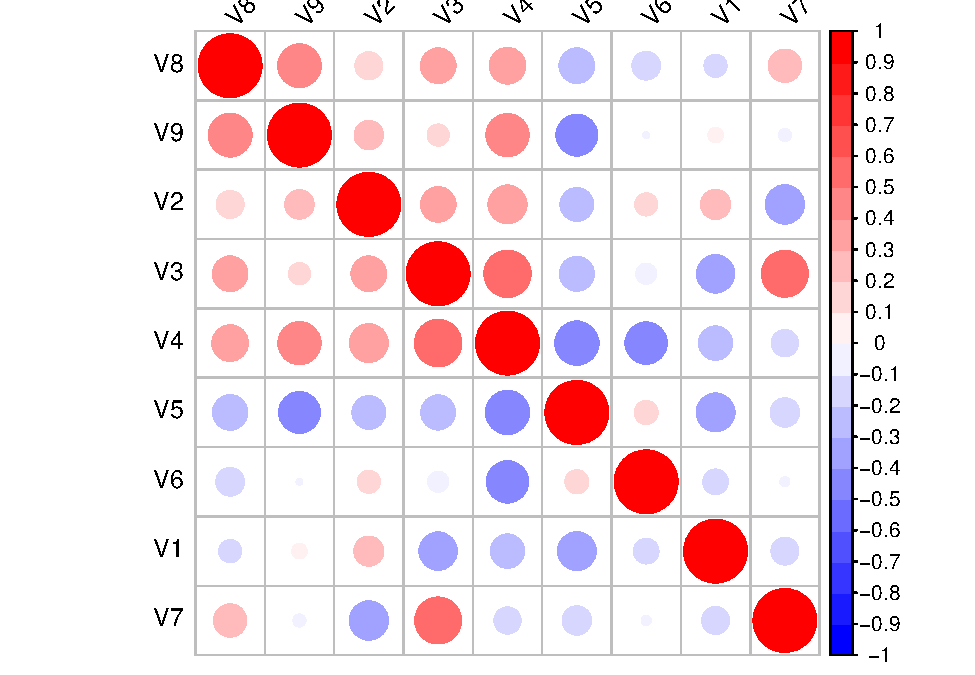
\includegraphics[width=0.65\linewidth,height=0.65\textheight]{Report_files/figure-latex/heatmap-1} 

}

\caption{Heatmap of correlated variables (v3, v4) and (v4, v7) look to be most correlated}\label{fig:heatmap}
\end{figure}
\begin{figure}

{\centering 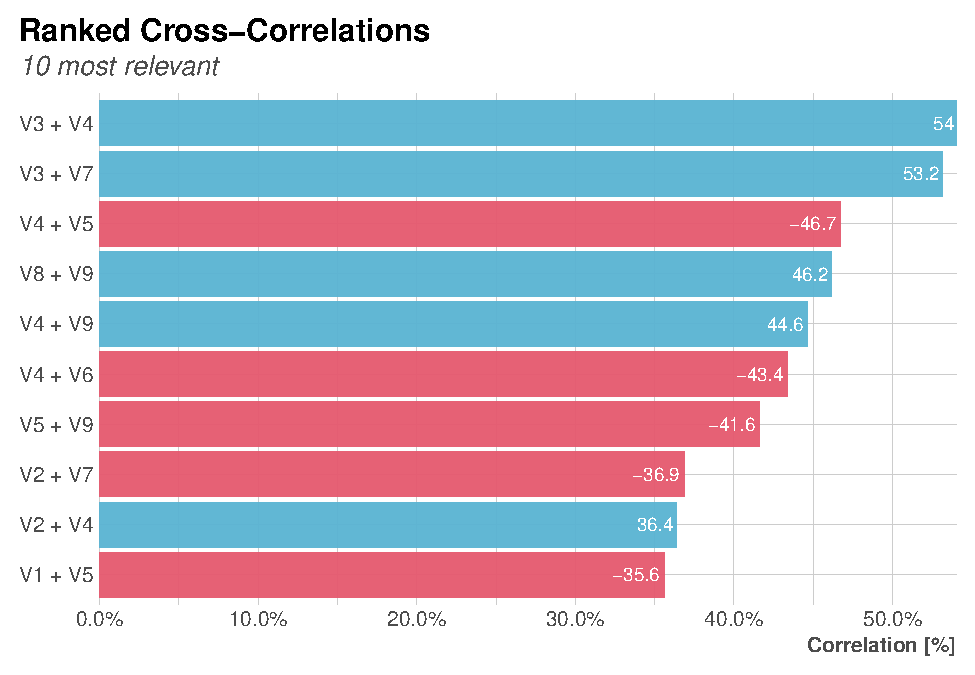
\includegraphics[width=0.65\linewidth,height=0.65\textheight]{Report_files/figure-latex/correlated_list-1} 

}

\caption{Ordered list of highest correlated pairs of variables}\label{fig:correlated_list}
\end{figure}

\textbf{Answer: }(v3, v4) are the most correlated with pearson
correlation value of 0.54

\hypertarget{what-is-the-trace-of-the-variance-matrix-of-your-data-set}{%
\subsubsection{3. What is the trace of the variance matrix of your data
set?}\label{what-is-the-trace-of-the-variance-matrix-of-your-data-set}}

\begin{Shaded}
\begin{Highlighting}[]
\NormalTok{covariance <-}\StringTok{ }\KeywordTok{cov}\NormalTok{(ass1[}\DecValTok{2}\OperatorTok{:}\DecValTok{10}\NormalTok{])}
\NormalTok{trace <-}\StringTok{ }\KeywordTok{sum}\NormalTok{(}\KeywordTok{diag}\NormalTok{(covariance))}
\NormalTok{trace}
\end{Highlighting}
\end{Shaded}

\begin{verbatim}
## [1] 55.92727
\end{verbatim}

\(trace = 55.93\)

\hypertarget{plot-the-points-on-the-first-two-principal-components}{%
\subsubsection{4. Plot the points on the first two principal
components}\label{plot-the-points-on-the-first-two-principal-components}}

\begin{figure}

{\centering 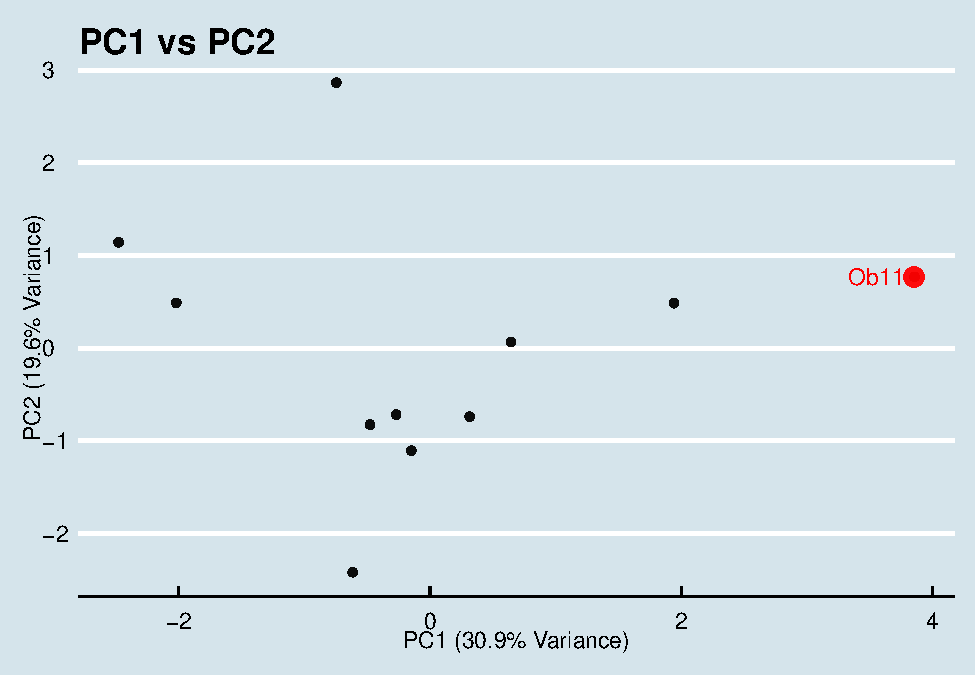
\includegraphics[width=0.65\linewidth,height=0.65\textheight]{Report_files/figure-latex/1.4-1} 

}

\caption{Scatter plot of PCA1 and PCA2}\label{fig:1.4}
\end{figure}

\hypertarget{what-proportion-of-the-information-in-the-data-set-is-given-by-the-first-4-principal-components}{%
\subsubsection{5. What proportion of the information in the data set is
given by the first 4 principal
components?}\label{what-proportion-of-the-information-in-the-data-set-is-given-by-the-first-4-principal-components}}

\textbackslash begin\{figure\}

\{\centering 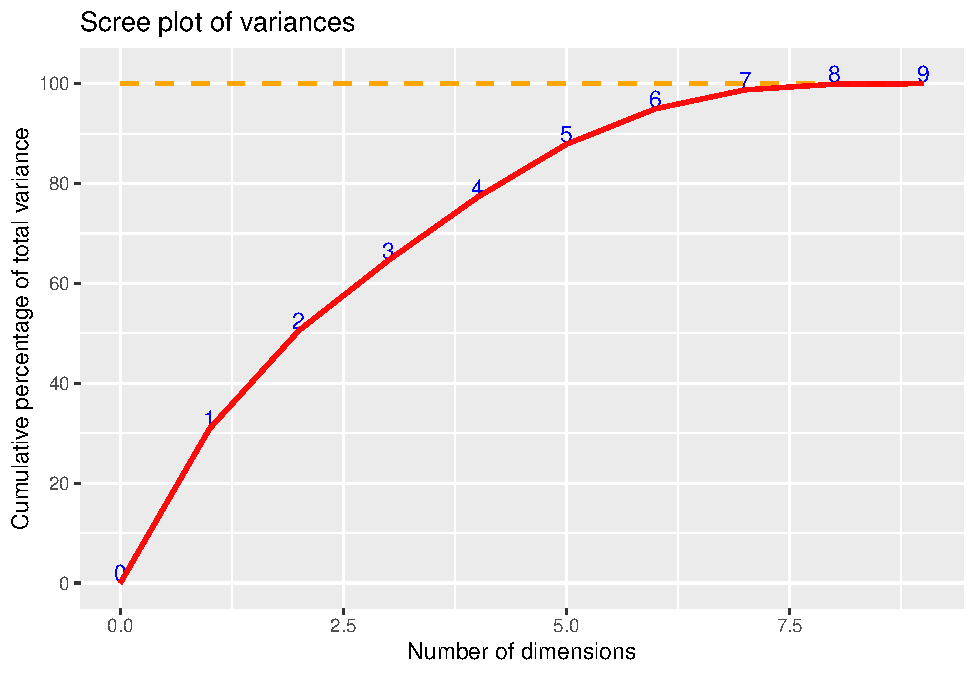
\includegraphics[width=0.65\linewidth,height=0.65\textheight]{Report_files/figure-latex/1.5-1}

\}

\textbackslash caption\{Scree plot shows first 4 components account for
\textasciitilde77\% of variance\}\label{fig:1.5}
\textbackslash end\{figure\}

\begin{verbatim}
## Importance of components:
##                           Comp.1    Comp.2    Comp.3    Comp.4    Comp.5
## Standard deviation     1.6682247 1.3288830 1.1234075 1.0673868 0.9794506
## Proportion of Variance 0.3092193 0.1962144 0.1402272 0.1265905 0.1065915
## Cumulative Proportion  0.3092193 0.5054337 0.6456609 0.7722514 0.8788429
##                            Comp.6     Comp.7     Comp.8     Comp.9
## Standard deviation     0.79975545 0.58246646 0.31896616 0.09898727
## Proportion of Variance 0.07106764 0.03769635 0.01130438 0.00108872
## Cumulative Proportion  0.94991055 0.98760690 0.99891128 1.00000000
\end{verbatim}

\textbf{Answer: }0.77

\hypertarget{lda}{%
\subsubsection{6. LDA}\label{lda}}

\begin{figure}

{\centering 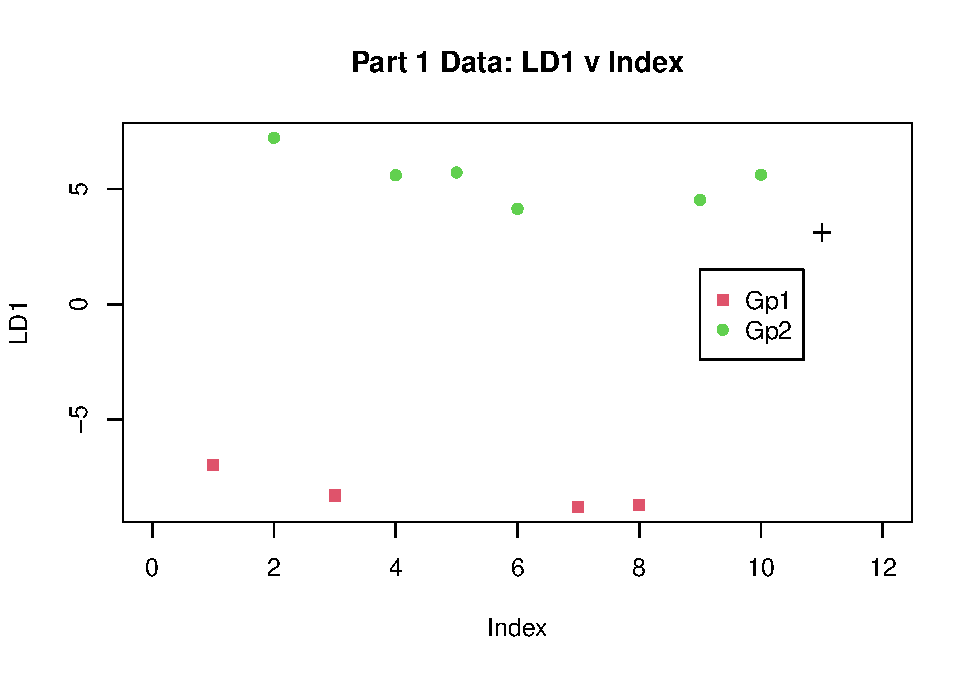
\includegraphics[width=0.65\linewidth,height=0.65\textheight]{Report_files/figure-latex/1.6-1} 

}

\caption{Plot of LDA against index of observations (LD2 not present). Cross-hair point at index = 11 shows the test data predicted as being, wrongly, in group 2, but it belongs to group 1}\label{fig:1.6}
\end{figure}

\begin{verbatim}
##       
## gptest 1 2
##      1 0 1
\end{verbatim}

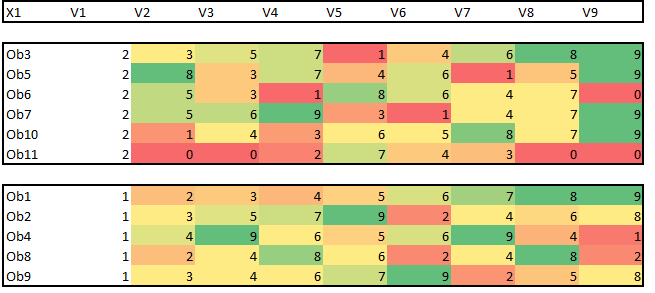
\includegraphics{1-6.png}

\textbf{Answer: } As seen from the last R output, The observation 1 is
in group 1, but it is predicted to be in group 2, hence the value of 1
in the 2 column.

From the excel table above (a comparison of the data between V1 values),
it looks as though that V9 is having a big sway on this, those in group
2 only have values of 0 and 9 for this variable, as does the first
observation, therefore it's wrongly placed into group 2. The group 1s
have values in between 1 and 8 inclusive.

\hypertarget{part-2}{%
\section{PART 2}\label{part-2}}

\hypertarget{determine-an-appropriate-number-of-principal-components}{%
\subsubsection{1. Determine an appropriate number of principal
components}\label{determine-an-appropriate-number-of-principal-components}}

\begin{verbatim}
## Importance of components:
##                           Comp.1    Comp.2    Comp.3    Comp.4    Comp.5
## Standard deviation     2.0299502 1.1563431 0.8610357 0.6491727 0.4310521
## Proportion of Variance 0.5886711 0.1910185 0.1059118 0.0602036 0.0265437
## Cumulative Proportion  0.5886711 0.7796896 0.8856014 0.9458050 0.9723487
##                            Comp.6      Comp.7
## Standard deviation     0.38275628 0.216925572
## Proportion of Variance 0.02092891 0.006722386
## Cumulative Proportion  0.99327761 1.000000000
\end{verbatim}

\begin{figure}

{\centering 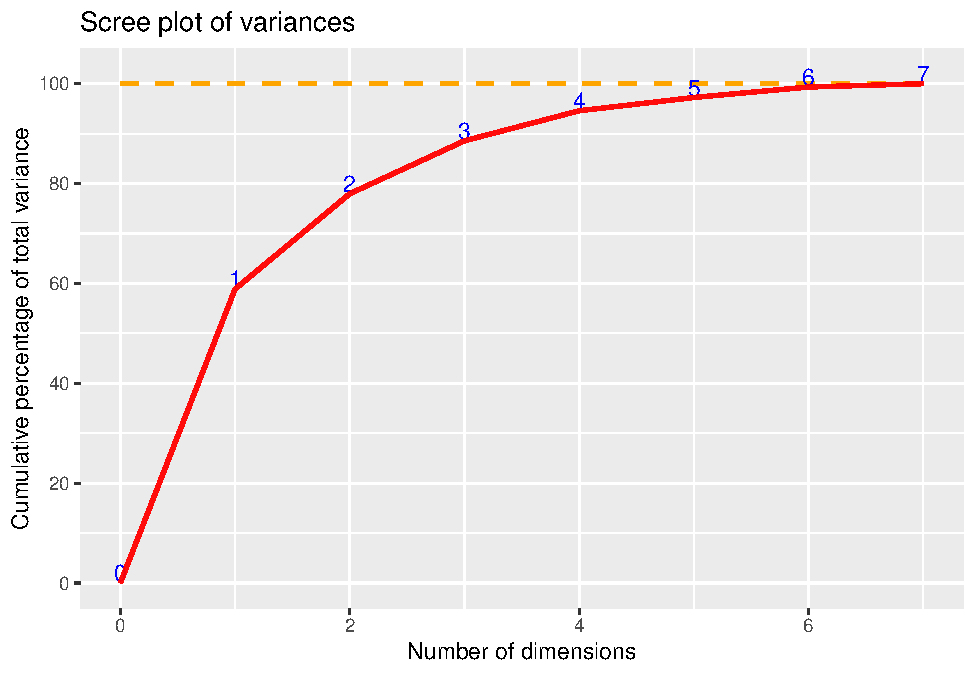
\includegraphics[width=0.65\linewidth,height=0.65\textheight]{Report_files/figure-latex/2.1-1} 

}

\caption{Scree plot showing a plateau at 4 PCAs}\label{fig:2.1}
\end{figure}

\textbf{Answer: } The jump from 2 to 3 PCAs explains \textasciitilde10\%
more variance, as does 3 to 4 PCAs, so no strong justification to drop
the 4th PCA. The jump from the 4th PCA to the 5th only provides an extra
\textasciitilde3\%, hence we see a pleatau in the figure and discard the
PCAs from 5 onwards

\hypertarget{give-a-description-of-the-main-sources-of-variation-of-the-quality-of-the-rubies}{%
\section{2 Give a description of the main sources of variation of the
quality of the
rubies}\label{give-a-description-of-the-main-sources-of-variation-of-the-quality-of-the-rubies}}

\begin{figure}

{\centering 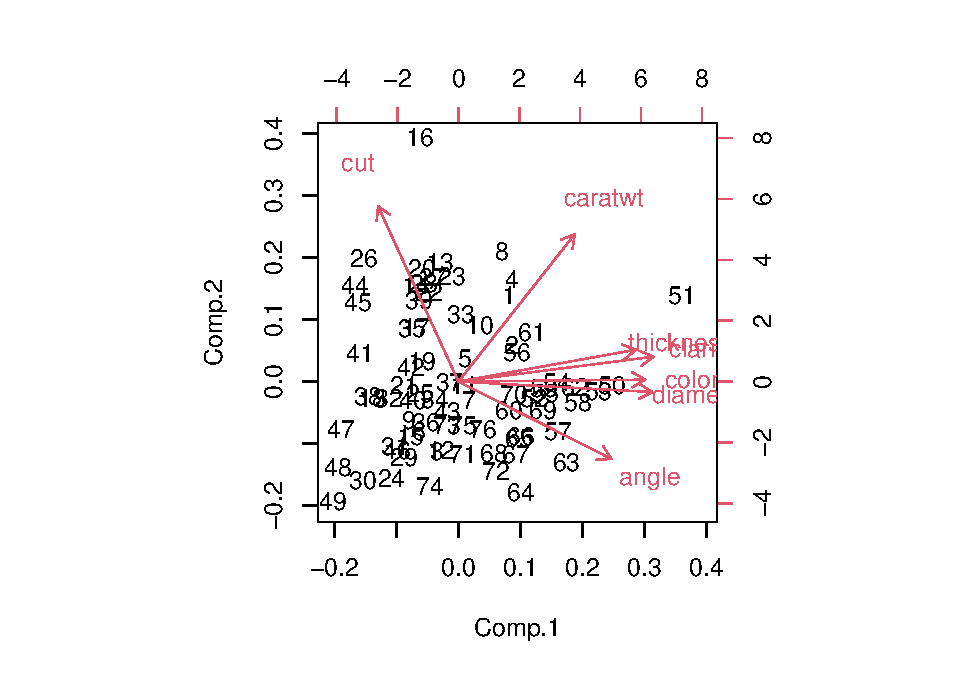
\includegraphics[width=0.65\linewidth,height=0.65\textheight]{Report_files/figure-latex/2.2-1} 

}

\caption{Biplot of PCA1 (Comp.1) vs PCA2 (Comp.2) }\label{fig:2.2}
\end{figure}

\begin{verbatim}
## 
## Loadings:
##           Comp.1 Comp.2 Comp.3 Comp.4 Comp.5 Comp.6 Comp.7
## color      0.434         0.452  0.243  0.143  0.434  0.582
## diameter   0.450         0.416  0.113               -0.775
## thickness  0.412  0.130 -0.450  0.247 -0.719  0.177       
## angle      0.356 -0.316 -0.568  0.315  0.579 -0.128       
## cut       -0.187  0.715         0.618  0.160 -0.208       
## clarity    0.453  0.101  0.177 -0.216 -0.110 -0.799  0.237
## caratwt    0.270  0.601 -0.253 -0.582  0.291  0.277       
## 
##                Comp.1 Comp.2 Comp.3 Comp.4 Comp.5 Comp.6 Comp.7
## SS loadings     1.000  1.000  1.000  1.000  1.000  1.000  1.000
## Proportion Var  0.143  0.143  0.143  0.143  0.143  0.143  0.143
## Cumulative Var  0.143  0.286  0.429  0.571  0.714  0.857  1.000
\end{verbatim}

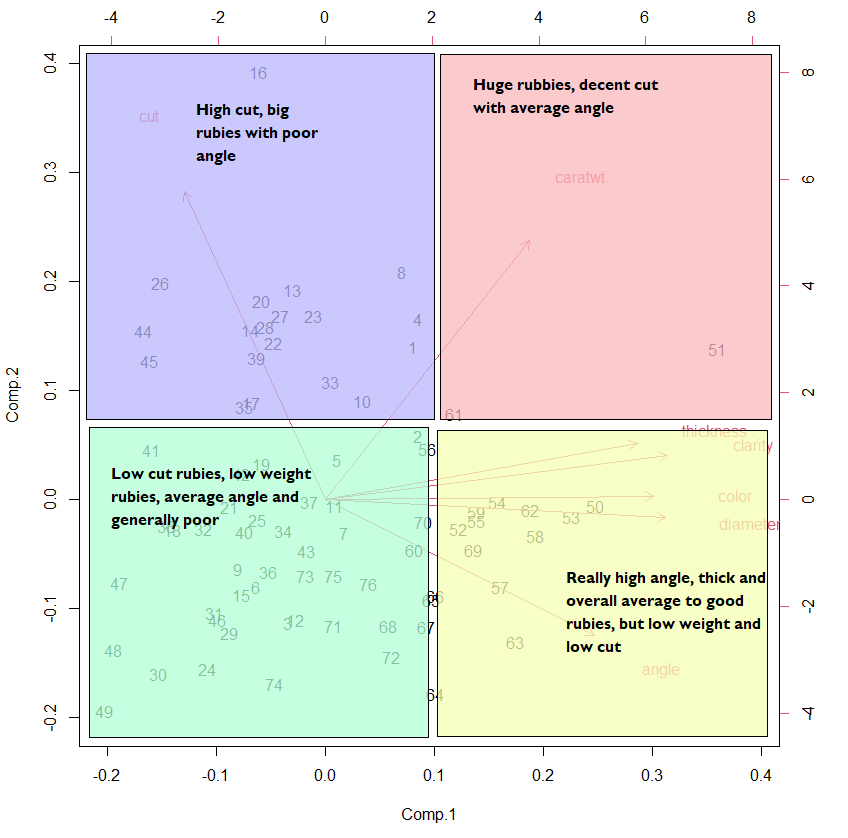
\includegraphics{2.2.png}

\textbf{Answer: } The first two PCAs account for \textasciitilde78\% of
the variance. Between the 2 PCAs, the cut accounts for a lot of the
variance. Using these PCAS, the data can be split up into 4 groups and
these properties account for the variance of quality. 1. High cut, big
rubies with poor angle 2. Huge rubies, lesser but still good cut, with
average angle 3. Low weight, low cut rubies, average angle and generally
poor quality. 4. Really high angle, thick and average to good rubies but
offset with a poor cut and lower weight rubies.

\hypertarget{what-are-the-characteristics-that-distinguish-the-three-countries-of-origin}{%
\section{3. What are the characteristics that distinguish the three
countries of
origin?}\label{what-are-the-characteristics-that-distinguish-the-three-countries-of-origin}}

\begin{figure}

{\centering 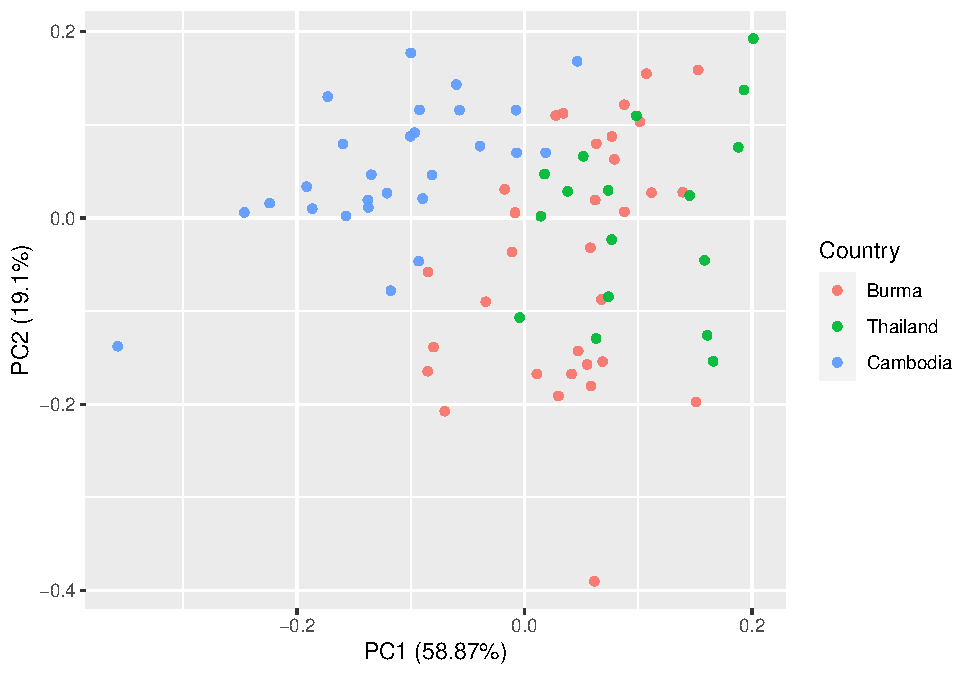
\includegraphics[width=0.65\linewidth,height=0.65\textheight]{Report_files/figure-latex/2.3-1} 

}

\caption{Biplot of PCA1 vs PCA2 with countries highlighted}\label{fig:2.3}
\end{figure}

This chart highlights where the rubies' from different countries sit in
the comparison of PC1 and PC2, however, in producing this chart the
signs of the loadings have been reversed, so we flip this image to
relate it to the first chart. (Couldn't find a way to reverse the
loadings values!)

\begin{figure}
\centering
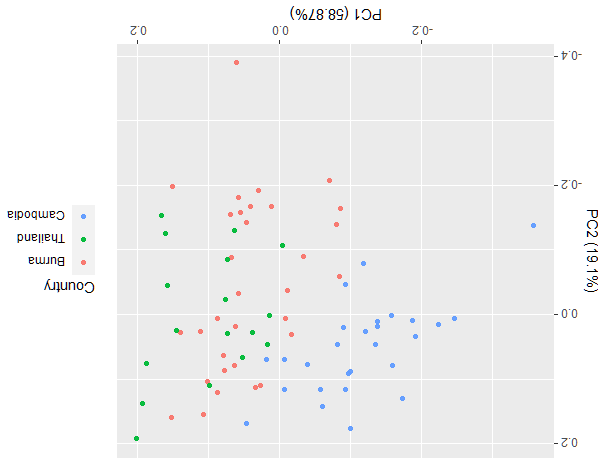
\includegraphics{2-3.png}
\caption{Comparison of the data between V1 values}
\end{figure}

\textbf{Burma} : Generally the rubies sit in the bottom left and top
left. A portion of Burmese rubies are poor, however a large portion of
rubies are also large with high cut, with average angle

\textbf{Thailand} : Generally low quality rubies with an average angle,
however some are bigger rubies with a high cut and poor angle. Similar
to Burmese rubies but poorer quality.

\textbf{Cambodia}: These rubies are generally good quality, scoring high
in many attributes with a high angle, and generally good shape. However
tend to be smaller and with a poor cut.

\hypertarget{outliers}{%
\section{4. Outliers}\label{outliers}}

Using the identify function, we see 2 outliers in row 16 and row 51.

\textbf{Observation 16} : The Burmese ruby scores a little below average
for the attributes except it has a maximum cut of 10 and one of the
heighest weights of 1.22, therefore we see it sit in the top left. It's
the ruby with the highest cut of 10, and the next highest is a distant
8, which makes it outlie so much. It's the 2nd biggest ruby, 2nd to the
next observation.

\textbf{Observation 51} : The Cambodian ruby scores really well in all
the attributes, except cut (4/10), and see its point on the far right of
the scatter plot. It is the thickest and best angled, most clear and
biggest rubies in the data. It's an outlier due to having the best
scores in 5 of the 7 attributes.

\hypertarget{and-6.-do-a-logistic-regression-and-discuss-how-successful-is-the-classification}{%
\section{5.and 6. Do a logistic regression and discuss how successful is
the
classification?}\label{and-6.-do-a-logistic-regression-and-discuss-how-successful-is-the-classification}}

For consistency, this analysis will not include price to serve as a
comparison with the PCA.

\begin{verbatim}
## 
## Call:
## glm(formula = where ~ color + diameter + thickness + angle + 
##     cut + clarity + caratwt, family = "binomial", data = df_log)
## 
## Deviance Residuals: 
##     Min       1Q   Median       3Q      Max  
## -1.9870  -0.6606  -0.3443   0.7039   1.8253  
## 
## Coefficients:
##              Estimate Std. Error z value Pr(>|z|)  
## (Intercept)   5.60591   12.91060   0.434   0.6641  
## color        -0.88368    1.29340  -0.683   0.4945  
## diameter      0.84586    0.90708   0.933   0.3511  
## thickness     0.39760    0.41758   0.952   0.3410  
## angle        -0.22174    0.09791  -2.265   0.0235 *
## cut          -0.47519    0.28890  -1.645   0.1000  
## clarity     -44.36438   18.40087  -2.411   0.0159 *
## caratwt       2.85172    4.52924   0.630   0.5289  
## ---
## Signif. codes:  0 '***' 0.001 '**' 0.01 '*' 0.05 '.' 0.1 ' ' 1
## 
## (Dispersion parameter for binomial family taken to be 1)
## 
##     Null deviance: 63.262  on 48  degrees of freedom
## Residual deviance: 43.520  on 41  degrees of freedom
## AIC: 59.52
## 
## Number of Fisher Scoring iterations: 5
\end{verbatim}

\begin{verbatim}
##    column.pred
##      0  1
##   0 28  4
##   1  8  9
\end{verbatim}

Here we have the output of the logistic regression and a table comparing
the predictions of the data vs the real values. The table shows there's
a good amount of bad predictions (non-column values). AIC, Null deviance
and Residual deviance are relatively low which indicates good
classification ability. The accuracy we see is 28 + 9/ 49 = 75\%
accuracy.

To further analyse how good it is at classifying new data, we split the
data into train and test data. For each country, 70\% of its data is
taken for training, and 30\% for testing.

\begin{verbatim}
## [1] "Confusion Matrix"
\end{verbatim}

\begin{verbatim}
##    columntest.pred
##     0 1
##   0 8 2
##   1 5 4
\end{verbatim}

\begin{verbatim}
## [1] "Sensitivity"
\end{verbatim}

\begin{verbatim}
## [1] 0.4444444
\end{verbatim}

\begin{verbatim}
## [1] "Specificity"
\end{verbatim}

\begin{verbatim}
## [1] 0.8
\end{verbatim}

\begin{verbatim}
## [1] "Accuracy"
\end{verbatim}

\begin{verbatim}
## [1] 0.6315789
\end{verbatim}

\begin{figure}

{\centering 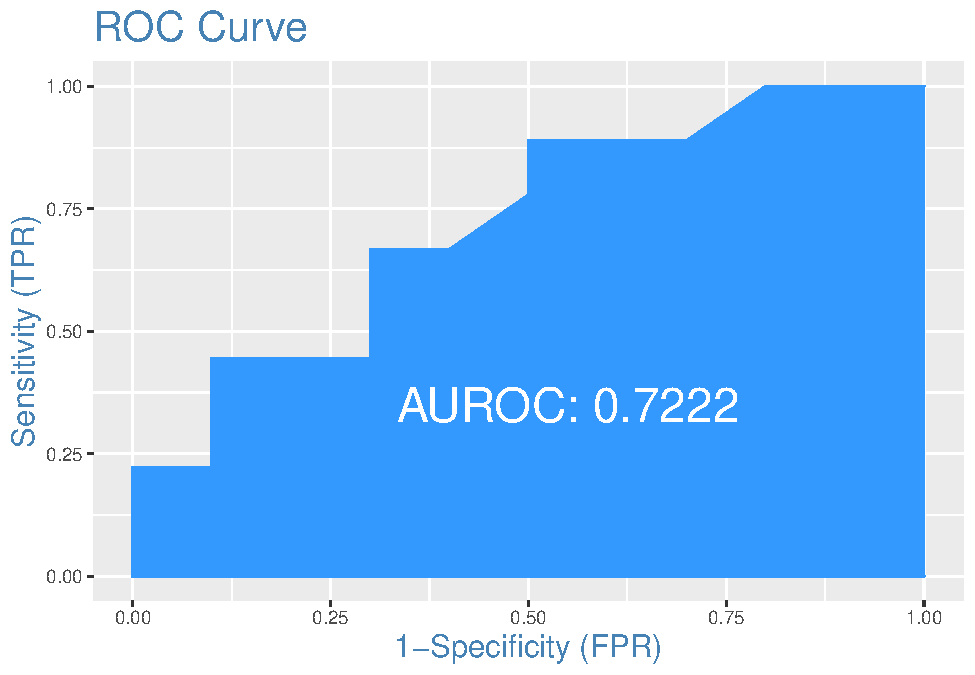
\includegraphics{Report_files/figure-latex/2.5a-1} 

}

\caption{ROC plot}\label{fig:2.5a}
\end{figure}

Sensitivity: \% Actual Thai correctly predicted to be Thai

Specificity: \% Actual Burmese correctly predicted to be Burmese

Accuracy of 63\% doesn't suggest it's a good model for classifying
rubies to countries, due to the low train size.

The AUC value of 0.72 suggests an acceptable ability to classify,
however it is not good.

The confusion matrix shows a poor ability to correctly classify.

The specificity suggests the model is good at classifying Burmese
rubies, but not the Thai rubies (low sensitivity).

Overall, it would be a mediocre model when it comes to predicting if a
ruby is Burmese or Thai.

\hypertarget{a.-classifying-new-ruby}{%
\section{7a. Classifying new ruby}\label{a.-classifying-new-ruby}}

\begin{verbatim}
##          1 
## 0.02360779
\end{verbatim}

This prediction is based off the regression using all the data and not
splitting it into train and test - in order to improve predictive power.

This ruby would be predicted to be a Burmese ruby as the probability is
closer to 0 (2.3\%).

\hypertarget{b.-predict-price-of-new-ruby}{%
\section{7b. Predict price of new
ruby}\label{b.-predict-price-of-new-ruby}}

We would do this using an OLS with price as the outcome variable

\begin{verbatim}
##        1 
## 451.6755
\end{verbatim}

The new ruby price is predicted as 451.68. One of the more expensive
rubies, in the top 25\% of the data.

\end{document}
